\documentclass[10 pt,usenames,dvipsnames, oneside]{article}
\usepackage{../../../modelo-ensino-medio}



\begin{document}

\begin{center}
  \begin{minipage}[l]{3cm}

\includegraphics[width=2cm]{logo}    
\end{minipage}\hfill
\begin{minipage}[r]{.8\textwidth}
 {\Large \scshape Atividade: Exploração de parâmetros da Função Seno}  
\end{minipage}
\end{center}
\vspace{.2cm}

\ifdefined\prof
%Habilidades da BNCC
% \begin{objetivos}
% \item 
% \end{objetivos}

%Caixa do Para o Professor
\begin{goals}
%Objetivos específicos
\begin{enumerate}
\item Reconhecer as transformações geométricas (translações,
reflexões, expansões e contrações horizontais ou verticais)
associadas a parâmetros aplicados às expressões analíticas
das funções seno e cosseno no esboço do seu gráfico.
\item Explorar o gráfico da função seno por meio do GeoGebra
\end{enumerate}

\tcblower

%Orientações e sugestões
No item \titem{c)} alteramos o parâmetro $b$ e perguntamos as implicações. Como o controle desliza de maneira contínua, não percebemos a principal diferença entre $f(x) = \sen(x)$ e $g(x)= \sen(-x)$. O aluno pode achar que a única diferença nesse parâmetro é no período, mas faça-os perceber que $\sen(x)=-\sen(-x)$
\end{goals}

\bigskip
\begin{center}
{\large \scshape Atividade}
\end{center}
\fi

Abra uma tela nova no GeoGebra e siga os seguintes passos:

\begin{enumerate}[label=\titem{\arabic*.}, left=0pt]
\item Crie controles deslizantes com nomes $a$, $b$, $c$ e $d$. Para isso, basta digitar no campo Entrada: $a=1$ e Enter; $b=1$ e Enter e assim por diante. O GeoGebra criará automaticamente os controles deslizantes.
  \begin{figure}[H]
  \centering
  
  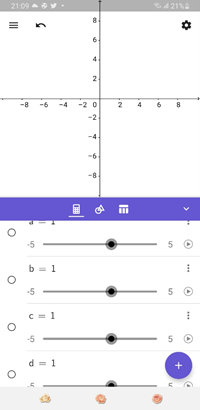
\includegraphics[width=.3\linewidth]{trigonometricas87}
  \end{figure}

\newpage
\item Digite no campo Entrada a função $y = a*sen(bx+c)+d$ e tecle Enter.
\begin{figure}[H]
  \centering
  
  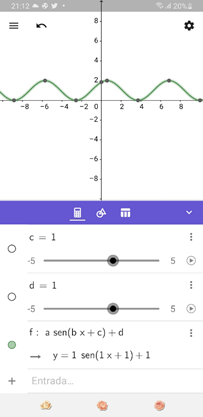
\includegraphics[width=.3\linewidth]{trigonometricas88}
  \end{figure}
 
\item Mova os controles deslizantes $a$ e $b$ para o valor $1$ e os controles $c$ e $d$ para zero. Se tiver dificuldade, você pode tocar sobre o valor do controle deslizante e fazer o ajuste digitando o valor desejado.
\begin{figure}[H]
  \centering
  
  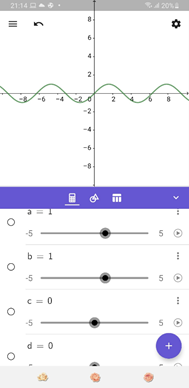
\includegraphics[width=.3\linewidth]{trigonometricas89}
  \end{figure}

\end{enumerate}
 
 \ifdefined\prof
 \clearpage
 \else
 \fi
\begin{enumerate}
\item Movimente lentamente o controle deslizante $a$ para a direita e para a esquerda. O que você observa? Registre suas observações. 
\item Retorne o controle deslizante $a$ para o valor $1$. Agora movimente lentamente o controle deslizante $b$ para a direita e para a esquerda. O que você observa? Registre suas observações.
\item Retorne o controle deslizante $b$ para o valor $1$. Agora movimente lentamente o controle deslizante $c$ para a direita e para a esquerda. O que você observa? Registre suas observações.
\item Retorne o controle deslizante $c$ para o valor $0$. Agora movimente lentamente o controle deslizante $d$ para a direita e para a esquerda. O que você observa? Registre suas observações.
\end{enumerate}

\ifdefined\prof
\begin{solucao}

\begin{enumerate}
\item Quando movemos o controle deslizante de forma que o valor de a seja positivo, a amplitude aumenta quando aumentamos o valor de $a$. Quando $a=0$ a função fica constante, igual a $d$; Quando os valores de a são negativos, a amplitude aumenta quando se aumenta o módulo de $a$ (ou seja, quando se move cada vez mais o controle para a esquerda). O gráfico da função que tem coeficiente $a = k$ é a reflexão, em torno do eixo dos $x$, do gráfico da mesma função quando $a = -k$.
\item Quando se aumenta o valor de $|b|$ diminui-se o período da função. Quando se diminui o valor de $|b|$, aumenta-se o período da função. Quando $b=0$, a função fica constante, igual a $a\cdot\sen(c)+d$.
\item Quando $c>0$, o gráfico se move para a esquerda; quando $c<0$, o gráfico se move para direita.
\item Quando $d>0$, o gráfico se move para cima; Quando $d<o$, o gráfico se move para baixo
\end{enumerate}

\end{solucao}
\fi

\end{document}